\documentclass{beamer}
% \usepackage{pgfpages}
% \pgfpagesuselayout{4 on 1}[a4paper,landscape,border shrink=5mm]
\usepackage{tikz}
\usetikzlibrary{shapes, backgrounds, arrows, positioning}
%\usepackage{pgfplots}
\usepackage{listings}
\usepackage[utf8,latin1]{inputenc}
\usepackage[natbibapa]{apacite}
\makeatletter \def\newblock{\beamer@newblock} \makeatother  

\beamertemplatenavigationsymbolsempty
\setbeamertemplate{itemize items}[circle]
\setbeamertemplate{section in toc}[circle]
\mode<beamer>{\setbeamercolor{math text displayed}{fg=iwmgrau}}
\setbeamercolor{block body}{bg=iwmorange!50!white}
\setbeamercolor{block title}{fg=white, bg=iwmorange}

\definecolor{iwmorange}{RGB}{255,105,0}
\definecolor{iwmgrau}{RGB}{67,79,79}
\setbeamercolor{title}{fg=iwmorange}
\setbeamercolor{frametitle}{fg=iwmorange}
\setbeamercolor{structure}{fg=iwmorange}
\setbeamercolor{normal text}{fg=iwmgrau}
\setbeamercolor{author}{fg=iwmgrau}
\setbeamercolor{date}{fg=iwmgrau}

\title{Multilevel Models}
\author{Nora Umbach%\footnote{These slides are a modified version of slides created by \url{https://osf.io/ /}. }
}
%\institute{\includegraphics[scale=.15]{figures/ut_logo}}
\date{June 28, 2021}
%\date{Last modified: \today}

\newcommand{\vect}[1]{\mathbf{#1}}
\newcommand{\mat}[1]{\mathbf{#1}}
\newcommand{\gvect}[1]{\boldsymbol{#1}}
\newcommand{\gmat}[1]{\boldsymbol{#1}}

\lstset{language=R,%
  literate={Ü}{{\"U}}1
           {ü}{{\"u}}1,
  %backgroundcolor=\color{iwmgrau!80!white},
  basicstyle=\ttfamily\color{iwmorange},
  frame=single,
  commentstyle=\slshape\color{black},
  keywordstyle=\bfseries\color{white},
  identifierstyle=\color{white},
  stringstyle=\color{green!85!black},
  numbers=none,%left,numberstyle=\tiny,
  basewidth={.5em, .4em},
  showstringspaces=false,
  emphstyle=\color{red!50!white}}

\lstdefinestyle{plain}{language=R,
  frame=none,
  basicstyle=\ttfamily\color{iwmorange},
  commentstyle=\slshape\color{iwmgrau},
  keywordstyle=\bfseries\color{iwmgrau},
  identifierstyle=\color{iwmgrau},
  stringstyle=\color{iwmgrau},
  numbers=none,
  basewidth={.5em, .4em},
  showstringspaces=false}

\pgfmathdeclarefunction{gauss}{2}{%
  \pgfmathparse{1/(#2*sqrt(2*pi))*exp(-((x-#1)^2)/(2*#2^2))}%
}

\AtBeginSection[]{
  \frame{
    \tableofcontents[sectionstyle=show/hide, subsectionstyle=show/show/hide]}}

\setbeamertemplate{headline}{
 \begin{beamercolorbox}{section in head}
   \vskip5pt\insertsectionnavigationhorizontal{\paperwidth}{}{}\vskip2pt
 \end{beamercolorbox}
}

\setbeamertemplate{footline}{\vskip-2pt\hfill\insertframenumber$\;$\vskip2pt}

\begin{document}

\begin{frame}{}
\thispagestyle{empty}
\titlepage
\end{frame}

% \begin{frame}{Outline}
% \tableofcontents
% \end{frame}

\begin{frame}[fragile]{Multilevel models}
  \begin{itemize}
    \item are special cases of mixed-effects models
    \item are useful for data with a hierarchical structure
    \item usually contain nested random effects
  \end{itemize}
  \vspace{1cm}
  We will look at an example from the book ``Practical Regression and
  Anova'' by Julian Faraway: the Junior School Project data
  \begin{lstlisting}[style=plain]
  library(faraway)
  data(jsp)
  ?jsp
  str(jsp)
  summary(jsp)
  head(jsp)
  \end{lstlisting}
\end{frame}

\begin{frame}{Junior School Project}
  A data frame with 3236 observations on the following 9 variables\\~\\

  \begin{tabular}{lp{8cm}}
    \hline
     \texttt{school} & 50 schools code 1--50 \\
     \texttt{class} & a factor with levels `1' `2' `3' `4' \\
     \texttt{gender} & a factor with levels `boy' `girl' \\
     \texttt{social} & class of the father I=1; II=2; III nonmanual=3; III
          manual=4; IV=5; V=6; Long-term unemployed=7; Not currently
          employed=8; Father absent=9 \\
     \texttt{raven} & test score \\
     \texttt{id} & student id coded 1--1402 \\
     \texttt{english} & score on English \\
     \texttt{math} & score on Maths \\
     \texttt{year} & year of school \\
     \hline
  \end{tabular}
  
  \flushright{\tiny{\url{https://en.wikipedia.org/wiki/Raven\%27s_Progressive_Matrices}}}
\end{frame}

{\setbeamercolor{background canvas}{bg=iwmgrau!80!white}

\begin{frame}[fragile]{Nested structure of data}
  \begin{lstlisting}
data(jsp)
str(jsp)
xtabs( ~ school + class, jsp, sparse=TRUE)

# Investigate nested structure of the data
xtabs( ~ school + factor(school:class), jsp,
  sparse=TRUE)

# Several data points per student
table(jsp$year, useNA="ifany")

dat <- subset(jsp, year == 0)
  \end{lstlisting}
\end{frame}

}

\begin{frame}[fragile]{Visualization of data}
  \begin{columns}
    \begin{column}{6cm}
      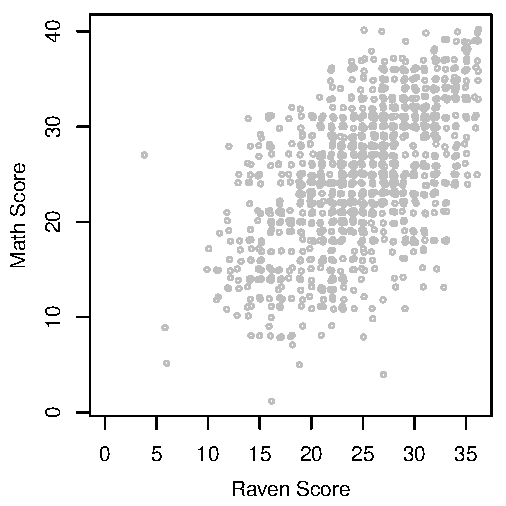
\includegraphics[scale=.8]{figures/jsp_scatter}
    \end{column}
    \begin{column}{4cm}
      \begin{lstlisting}[style=plain]
plot(math ~ raven, dat,
  xlab="Raven Score", 
  ylab="Math Score")
      \end{lstlisting}
    \end{column}
  \end{columns}
\end{frame}

\begin{frame}[fragile]{Visualization of data}
  \begin{columns}
    \begin{column}{6cm}
      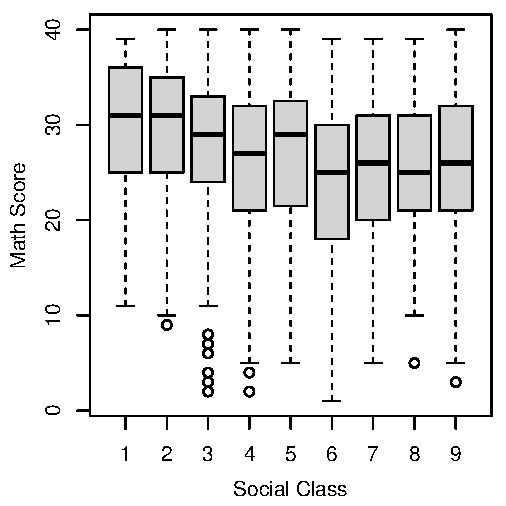
\includegraphics[scale=.8]{figures/jsp_box1}
    \end{column}
    \begin{column}{4cm}
      \begin{lstlisting}[style=plain]
plot(math ~ social, dat,
  xlab="Social Class",
  ylab="Math Score")
      \end{lstlisting}
    \end{column}
  \end{columns}
\end{frame}

\begin{frame}[fragile]{Centering variables}
  \begin{itemize}
    \item Psychological variables often do not have a ``natural'' zero and
      linear transformations of the form $y = a\cdot x + b$, with $a$ and
      $b$ being constants, are allowed
    \item $x - \bar x$ is a linear transformation with $a = 1$ and $b =
      -\bar x$; this transformation is called centering of a variable
      (compare $z$ transformation)
    \item By centering variables the interpretation of the intercept in a
      linear model changes
    \begin{itemize}
      \item Uncentered intercepts represent the difference to a value of 0
      \item Centered intercepts represent the difference to the mean
    \end{itemize}
  \end{itemize}
\end{frame}

\begin{frame}{Centering variables}
  Options to center variables in multilevel models with two levels
  \begin{itemize}
    \item Level 1
      \begin{itemize}
        \item Centering around group mean
        \item Centering around grand mean
      \end{itemize}
    \item Level 2
      \begin{itemize}
        \item Centering around grand mean
      \end{itemize}
    \item Interpretation of the intercepts needs to refer to the respective
      value of 0 (point of origin)
    \item Attention
      \begin{itemize}
        \item Centering around the respective group mean might eliminate
          possible group differences between the group means
        \item In order to avoid this pitfall a variable that contains the
          group means should be included
      \end{itemize}
  \end{itemize}
\end{frame}

{\setbeamercolor{background canvas}{bg=iwmgrau!80!white}

\begin{frame}[fragile]{Centering of raven score}
  \begin{lstlisting}
# Centering around grand mean
dat$craven <- dat$raven - mean(dat$raven)

lm1 <- lm(math ~ raven, dat)
lm2 <- lm(math ~ craven, dat)

# Visualization
plot(jitter(math) ~ jitter(raven), dat, cex=.7, 
  xlab="Raven score", ylab="Math score", 
  xlim=c(0, 36), col="gray")
abline(v = 0, h = coef(lm1)[1], col="darkgray")
abline(v = mean(dat$raven), h = coef(lm2)[1],
  col="darkgray")
abline(lm1)
  \end{lstlisting}
\end{frame}

\begin{frame}[fragile]{Centering of raven score}
  \begin{lstlisting}
# Centering around group mean for each school
## add mean raven score per school
dat$mraven <- with(dat, ave(raven, school))
dat$mraven <- dat$mraven - mean(dat$mraven)
## center raven score: mean=0 for each school
dat$gcraven <- dat$craven - dat$mraven

aggregate(craven ~ school, dat, mean)
aggregate(gcraven ~ school, dat, mean)

# Visualization
plot(jitter(math) ~ jitter(craven), dat, cex=.7, 
  xlab="Centered raven score", ylab="Math score", 
  col="gray")
abline(v = unique(dat$mraven), col="lightblue")
abline(v = mean(dat$craven), col="blue", lwd=2)
  \end{lstlisting}
\end{frame}

}

\begin{frame}[fragile]{Visualization of data -- Schools}
  \begin{columns}
    \begin{column}{7cm}
      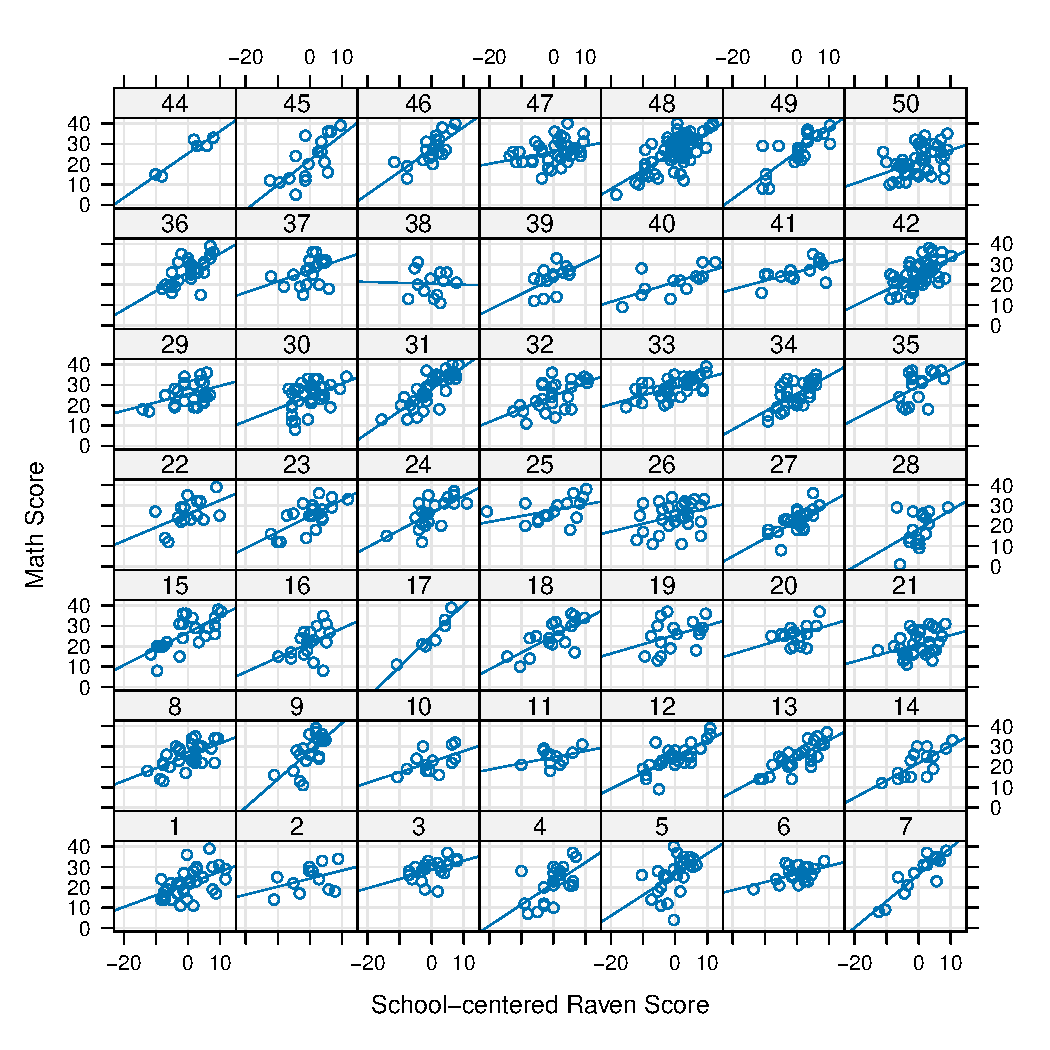
\includegraphics[scale=.4]{figures/jsp_lattice1}
    \end{column}
    \begin{column}{5cm}
      \begin{lstlisting}[style=plain]
library(lattice)

xyplot(
  math ~ gcraven | school,
  data=dat,
  xlab="Raven Score",
  ylab="Math Score",
  type=c("p", "g", "r")
)
      \end{lstlisting}
    \end{column}
  \end{columns}
\end{frame}

\begin{frame}[fragile]{Visualization of data -- Classes}
  \begin{columns}
    \begin{column}{15cm}
      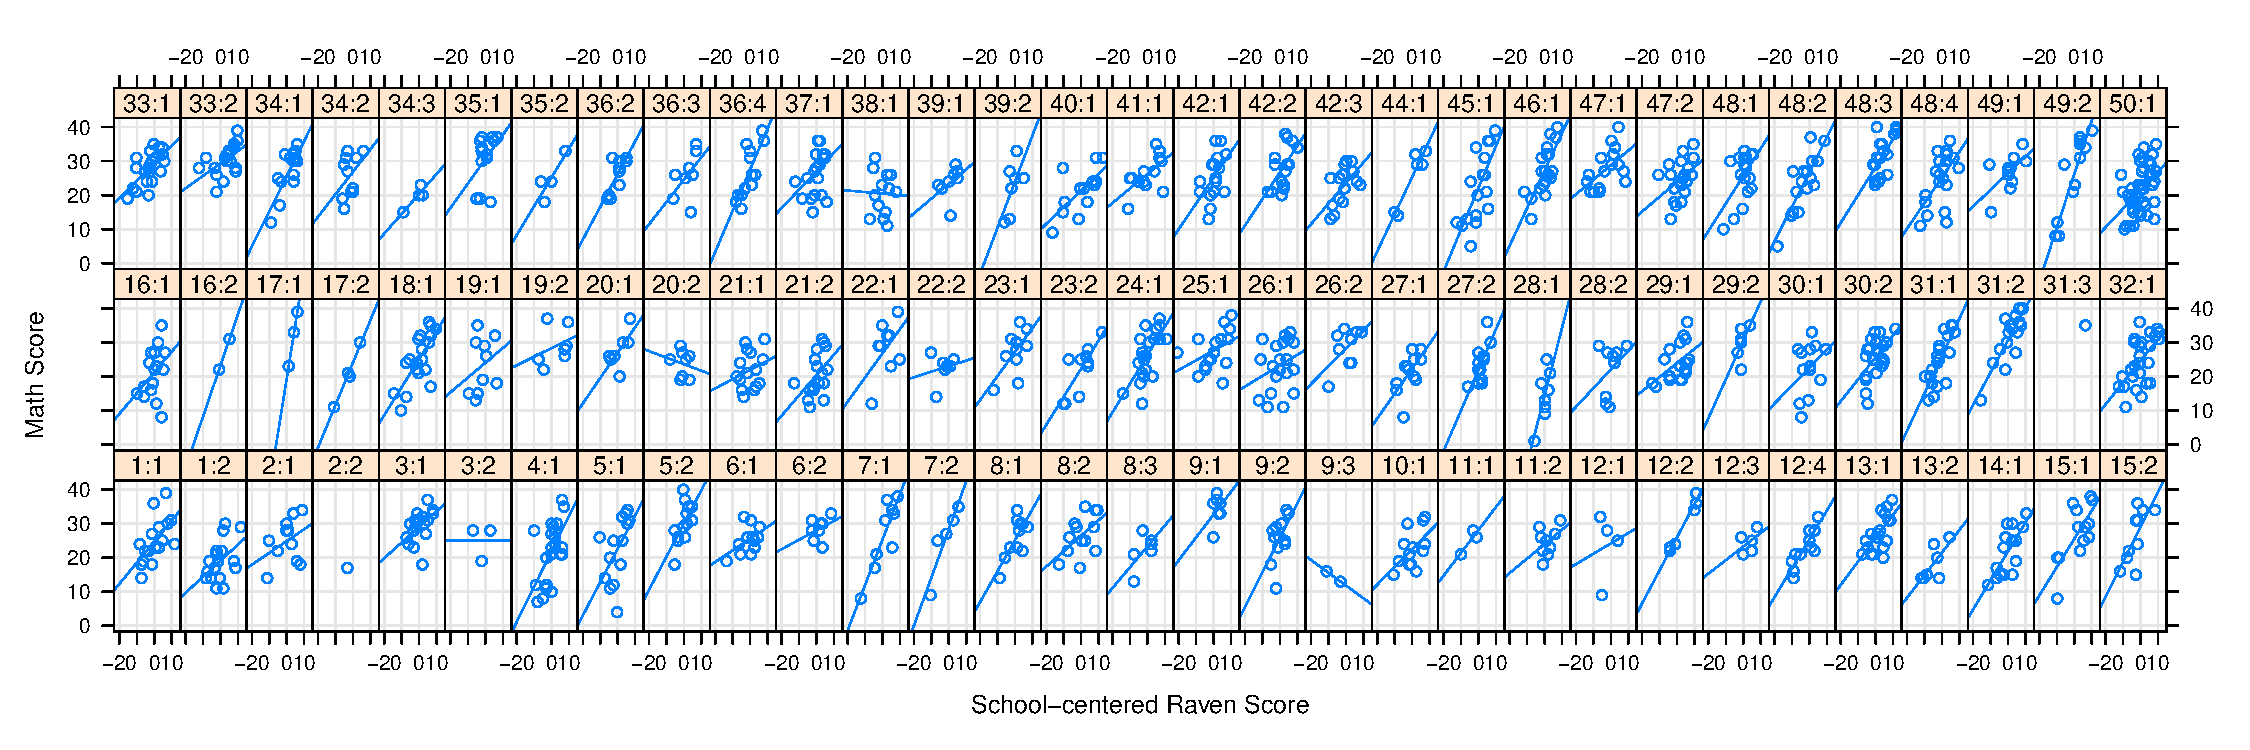
\includegraphics[scale=.34]{figures/jsp_lattice2}
    \end{column}
  \end{columns}
\begin{lstlisting}[style=plain]
xyplot(
  math ~ gcraven | school:class, data=dat,
  xlab="Raven Score", ylab="Math Score", 
  type=c("p", "g", "r")
)
\end{lstlisting}

\end{frame}

\begin{frame}{Random intercept model}
  \begin{itemize}
    \item The data actually consist of 3 levels: students in classes in
      schools
    \item Because there are no class-level predictors, the class effect
      $\omega$ enters on the same level as the school effect $\upsilon$
  \end{itemize}
\begin{align*}
\text{(Level 1)} \quad y_{ijk} &= b_{0ij} + b_{1i}\,gcraven_{ijk} + b_{2i}\,social_{ijk}\\
                  &~~~+ b_{3i}\,(gcraven_{ijk} \times social_{ijk}) +
                  \varepsilon_{ijk}\\
  \text{(Level 2)} \quad b_{0ij} &= \beta_0 + \upsilon_{0i} + \omega_{0j}\\
                  \quad b_{1i} &= \beta_1\\
                  \quad b_{2i} &= \beta_2\\
                  \quad b_{3i} &= \beta_3\\
\text{(2) in (1)} \quad y_{ijk} &= \beta_{0} + \beta_{1}\,gcraven_{ijk} +
  \beta_{2}\,social_{ijk}\\
                              &~~~ + \beta_{3}\,(gcraven_{ijk} \times social_{ijk})\\
                              &~~~ + \upsilon_{0i} + \omega_{0j} +
                              \varepsilon_{ijk}
\end{align*}
  \hspace{-.1cm}with $\upsilon_{0i} \sim N(0, \sigma^2_{\upsilon})$ i.i.d.,
$\omega_{0j} \sim N(0, \sigma^2_{\omega})$ i.i.d.,
$\varepsilon_{ijk} \sim N(0, \sigma^2)$ i.i.d.
\end{frame}

{\setbeamercolor{background canvas}{bg=iwmgrau!80!white}

\begin{frame}[fragile]{Random intercept model}
  \begin{lstlisting}
lme1 <- lmer(math ~ gcraven*social + (1 | school) + 
  (1 | school:class), dat, REML=F)
confint(lme1)

# Significance tests
lme0 <- lmer(math ~ 1 + (1 | school) + 
  (1 | school:class), dat, REML=F)
lme0.1 <- lmer(math ~ gcraven + (1 | school) + 
  (1 | school:class), dat, REML=F)
lme0.2 <- lmer(math ~ gcraven + social + 
  (1 | school) + (1 | school:class), dat, REML=F)
anova(lme0, lme0.1, lme0.2, lme1)

# Model diagnostics
plot(lme1)
qqnorm(resid(lme1)); qqline(resid(lme1))
  \end{lstlisting}
\end{frame}

}

\begin{frame}{Multilevel structure}
  We consider two levels:
  \begin{itemize}
    \item Level 1 refers to the students
    \item Level 2 refers to the schools
  \end{itemize}
  \vspace{.5cm}
    \begin{tabular}{llp{8cm}}
      Level & Variable & Description \\
    \hline
      2 & \texttt{school} & 50 schools code 1--50 \\
      2 & \texttt{mraven} & mean raven score of school (overall mean 0) \\
      %-- & \texttt{class} & a factor with levels `1' `2' `3' `4' \\
      1 & \texttt{social} & class of the father (categorical) \\
      1 & \texttt{raven} & test score \\
      1 & \texttt{gcraven} & centered test score (mean for each school 0)\\
      1 & \texttt{math} & score on Maths \\
     \hline
  \end{tabular}
\end{frame}

\begin{frame}{Multilevel structure}
\begin{align*}
\text{(Level 1)} \quad y_{ij} &= b_{0i} + b_{1i}\,gcraven_{ij} + b_{2i}\,social_{ij}\\
                            &~~~ + b_{3i}\,(gcraven_{ij}\times social_{ij}) + \varepsilon_{ij}\\
\text{(Level 2)} \quad b_{0i} &= \beta_0 + \beta_4\,mraven_i + \upsilon_{0i} \\
                 \quad b_{1i} &= \beta_1 + \beta_5\,mraven_i + \upsilon_{1i}\\
                 \quad b_{2i} &= \beta_2\\
                 \quad b_{3i} &= \beta_3\\
\text{(2) in (1)} \quad y_{ij} &= \beta_{0} + \beta_{1}\,gcraven_{ij} + \beta_{2}\,social_{ij}\\
                            &~~~ + \beta_{3}(gcraven_{ij}\times social_{ij}) + \beta_{4}\,mraven_i\\
                            &~~~ + \beta_{5}\,(gcraven_{ij} \times mraven_{i})\\
                            &~~~ + \upsilon_{0i} + \upsilon_{1i}\,gcraven_{ij} + \varepsilon_{ij}
\end{align*}
with $\gvect\upsilon \sim N(\gvect 0, \gmat{\Sigma}_\upsilon)$ i.i.d.,
$\varepsilon_{ij} \sim N(0, \sigma^2)$ i.i.d.
\end{frame}

{\setbeamercolor{background canvas}{bg=iwmgrau!80!white}

\begin{frame}[fragile]{Fitting multilevel model}
  \begin{lstlisting}
lme2 <- lmer(math ~ mraven*gcraven + gcraven + 
  (gcraven | school), dat, REML=F)

lme3 <- lmer(math ~ mraven*gcraven + gcraven + social +
  (gcraven | school), dat, REML=F)

lme4 <- lmer(math ~ mraven*gcraven + gcraven*social + 
  (gcraven | school), dat, REML=F)

anova(lme2, lme3, lme4)

summary(lme3)
confint(lme3)
  \end{lstlisting}
\end{frame}

}

\begin{frame}{Interpretation of results}
Fixed effects
  \begin{itemize}
    \item The mean math score for a student with mean intelligence in a
          mean intelligent school in the highest social class is 25.79
    \item By partitioning $craven = mraven + gcraven$, we can consider how
      intelligence affects math score on different levels
      \begin{itemize}
        \item If the mean raven score per school increases by one point,
          the math score increases by 0.62 (95\,\% CI: [0.37, 0.88])
        \item If the raven score for a student increases by one point, the
          math score increases by 0.69 (95\,\% CI: [0.61, 0.78])
      \end{itemize}
  \end{itemize}
\end{frame}

\begin{frame}{Interpretation of results}
Random effects
  \begin{itemize}
    \item We get an estimate of $\hat \sigma^2_{\upsilon_{0}} = 2.14$ for
      the variance of the mean math scores; this leaves room for improving
      the prediction by adding more school-level predictors
    \item There is hardly any variance for the dependence of math score on
      the raven score between schools ($\hat \sigma^2_{\upsilon_{1}} =
      0.03$); this should be kept in mind when interpreting the correlation
      of $\hat \rho_{\upsilon_{0}\upsilon_1} = -0.06$ (95\,\% CI: [-0.56,
      0.47])
    \item The corresponding covariance is $\hat
      \sigma_{\upsilon_{0}\upsilon_1} = -0.06 \cdot \hat
      \sigma_{\upsilon_{0}} \cdot \hat \sigma_{\upsilon_{1}} = -0.001$
    \item These results imply that a simpler model without random slopes for
      $gcraven$ within schools might fit the data
  \end{itemize}
\end{frame}


% {\setbeamercolor{background canvas}{bg=iwmgrau!80!white}
% 
% \begin{frame}[fragile]{}
%   \begin{lstlisting}
%   ##
%   \end{lstlisting}
% \end{frame}
% 
% }
% 
% \begin{frame}[fragile]{}
%   \begin{block}{Exercise}
%     \begin{itemize}
%       \item 
%     \end{itemize}
%   \end{block}
% \end{frame}

% \appendix
% %\begin{frame}[allowframebreaks]{References}
% \begin{frame}{References}
% %\renewcommand{\bibfont}{\footnotesize}
% \bibliographystyle{apacite}
% \bibliography{../../../literature/nu}
% \vfill
% \end{frame}

\end{document}

